\section{研究内容}
\label{sec:intro:work}

\subsection{主要内容}
\label{sec:intro:work:mainwork}

随着VoLTE商用范围的扩大,研究VoLTE环境中时间隐通道构建方法,既扩充了时间隐通道构建方法,也扩展了对VoLTE音视频通话特征的研究。本文主要研究在VoLTE视频通话场景下,通过主动丢包的方式,构建鲁棒的时间隐通道。本文主要包括四个研究点,分别为VoLTE主动丢包时间隐通道的检测方法、基于Zigzag映射矩阵的时间隐通道构建方法、基于多重校验纠错的时间隐通道构建方法,以及基于Linphone的时间隐通道原型系统。各研究点与研究指标的关联关系如图\nref{fig:1:contents}。

\insertFigure{
	\begin{figure}[htbp]
		\centering
        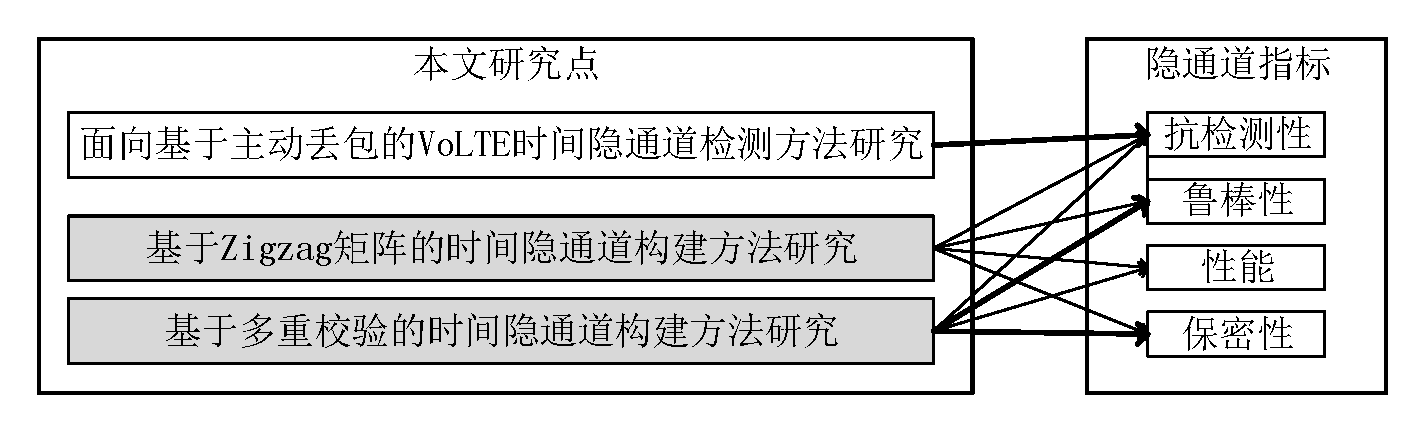
\includegraphics[width=0.95\textwidth]{chapters/chapter1/figures/struct.pdf}
        \caption{本文研究点与时间隐通道指标的对应关系}\label{fig:1:contents}
	\end{figure}
}

%背景介绍了什么
背景及相关工作部分,主要介绍了本文工作的研究基础,以及国内外研究现状。内容包括对现有时间隐通道构建方法的分析,涵盖了以太网中的构建方法、移动互联网中的构建方法,以及常用的鲁棒性策略。对VoLTE音视频传输方案的分析,分析了数据采集、处理、传输、呈现流程,并分析了音视频处理流程的差异。通过分析VoLTE传输协议,研究丢包对传输过程产生的影响,并结合随机字段提高保密性。抗检测能力是时间隐通道的重要指标,通过分析现有的时间隐通道检测方法,研究可用于检测主动丢包时间隐通道的方法。最后,总结时间隐通道应满足的指标。

%检测方法介绍了什么
VoLTE主动丢包时间隐通道的检测方法,主要研究在VoLTE场景下,如何有效检测基于主动丢包的时间隐通道。为筛选有效的检测模式,首先分析VoLTE通话的统计特征,包含丢包率、IPD、连续丢包数及区间丢包数几个方面。根据分析结果,结合不同维度的统计分析工具,汇总得到VoLTE主动丢包时间隐通道的检测方法。最后,通过模拟测试,测试检测方法的准确率。

%Zigzag方法说了什么
基于Zigzag映射矩阵的时间隐通道构建方法,研究基于Zigzag矩阵构建时间隐通道,同时在抗检测性、鲁棒性及传输性能之间实现均衡。按照研究背景和动机、隐通道构建方法介绍及隐通道评估结果为顺序展开,对该方法的研究基础、架构设计、调制解调方法及实验测试结果分别进行介绍。经过实验测试证明,通过调整传输参数,该时间隐通道达到了设计要求,具有良好的测试结果。

%多重校验方法说了什么
基于多重校验纠错的时间隐通道构建方法,重点研究如何进一步降低误码率,提高传输鲁棒性。该时间隐通道构建方法中,设计了包括码字间校验、码字自校验以及符号校验三级校验模式,结合映射矩阵提高鲁棒性。该部分由研究背景和动机开始,然后介绍该方法的构建架构,接下来逐层展开多重校验纠错方法。最后评估结果表明,该时间隐通道的鲁棒性有了较大提升。

%Linphone中验证说了什么
基于Linphone的时间隐通道原型系统,通过搭建原型系统并进行传输测试,检验主动丢包方法的可行性。基于Linphone平台,通过添加UI层隐通道控制接口、SDK层消息传输接口,以及oRTP层隐通道执行组件,实现时间隐通道原型系统的功能。通过实际传输测试评估,主动丢包的数据传输模式有效,具有有效的数据传输能力。

%以上各部分是怎样在逻辑上串起来的
背景及相关工作的介绍,分析出VoLTE视频通话场景下,通过主动丢包的方式构建时间隐通道是可行的。与此同时,现有的检测方法及鲁棒性方法,无法满足这种隐通道构建方式。VoLTE主动丢包时间隐通道的检测方法研究,着重解决如何检测主动丢包时间隐通道,同时也为本文提出的构建方法提供抗检测能力评估依据。接下来,提出了两种不同的时间隐通道构建方法,以不同的方式提高鲁棒性,并在实验评估中得到了较好结果。最终,基于Linphone平台构建原型系统进行传输测试,验证主动丢包的可行性。以上各部分结合起来,即为基于主动丢包的VoLTE时间隐通道构建方法研究的前提、检测方法、构建方法,以及原型验证。

\subsection{主要创新点}
\label{sec:intro:work:inno}

本文的研究重点,是在VoLTE场景下,通过主动丢包方式构建时间隐通道,同时提出检测方法以评估抗检测能力。主要的创新点包括以下四点:

\begin{enumerate}
    \item 提出了一种VoLTE场景中,对基于主动丢包时间隐通道的检测方法。该方法以统计分析为基础,综合多种量化评估方法,结合IPD及丢包特征两个维度进行检测判别。传统的时间隐通道检测方法,主要基于IPD分布进行检测识别,对基于主动丢包的时间隐通道来说不够全面。本方法完善了时间隐通道检测方法,经过实验测试,该检测方法能够检测出主动丢包率高于{0.4\ \%}的时间隐通道。
    \item 提出了一种基于Zigzag映射矩阵的时间隐通道构建方法,结合了基于CRC的码字校验方法,以及基于Zigzag映射矩阵的码字-符号转换。该方法的设计简单高效,以轻量级校验保证传输性能和鲁棒性。实验结果表明,该方法具有良好的抗检测能力,传输性能可达到{0.88\ bps},并且误码率保持在{1.5\ \%}左右,同时具有较小的构建代价。
    \item 提出了一种基于多重校验纠错的时间隐通道构建方法,重点研究如何通过逐级纠错的方式,降低噪声对时间隐通道的干扰。该方法的核心,是在不同的处理阶段引入相互独立的校验方式,在解调过程中逐级剔除噪声干扰,最终得到正确概率最高的消息。此外,通过引入可调映射矩阵,将连续丢包事件分散处理,减小连续丢包对纠错过程的干扰。经实验测试评估,该方法在传输速率达到{0.49\ bps}时,误码率不高于{0.08\ \%},鲁棒性得到有效提升。
    \item 基于Linphone平台,构建了时间隐通道原型系统。Linphone与VoLTE采用相同的SIP(Session Initiation Protocol)+RTP通话模式,通过在Linphone中构建基于主动丢包的时间隐通道,验证构建方法与网络环境的兼容性。传输测试结果表明,主动丢包方法具有有效的数据传输能力。
\end{enumerate}

\subsection{组织结构}
\label{sec:intro:work:struct}

全文共分六章,文章的组织结构如下:
\begin{itemize}
    \item 第1章,对本文的研究领域及主要内容进行介绍。
    \item 第2章,介绍本文中涉及的研究背景,以及国内外相关工作。内容包含研究基础、隐通道构建方法及检测方法方面的研究成果,以及时间隐通道应当满足的指标。
    \item 第3章,介绍VoLTE主动丢包时间隐通道的检测方法,通过结合多种特征及多种检测工具,提高隐通道检测能力。该检测方法,同时用于评估本文中构建方法的抗检测能力。
    \item 第4章,介绍基于Zigzag映射矩阵的时间隐通道构建方法,包含研究背景和动机、整体设计方案、实验及评估结果几部分。
    \item 第5章,介绍基于多重校验纠错的时间隐通道构建方法,包含背景和动机、隐通道整体设计方案、各层次鲁棒性方法,以及实验测试评估结果几部分。
    \item 第6章,介绍基于Linphone的时间隐通道原型系统,包含Linphone的基本结构、隐通道的模块以及关联关系,以及传输测试结果几部分。
\end{itemize}